\section{Theorie}

In dem Folgenden Versuch sollen die bei Einwirken eines Magnetfeldes auf ein Atom
entstehende Aufspaltung und Polarisation von emittierten Spektrallinien untersucht
werden. Dies geschieht anhand der blauen und roten Spektrallinien einer
Cadmium Lampe.

Der Effekt ist benannt nach dem Holländer P. Zeeman (1865-1945), welcher diese
Erscheinung 1896 erstmals am Licht eine Na-Lampe beobachtete.

\subsection{Das magnetische Moment}

Aufgrund der Quantenmechanik ist bekannt, dass jedes Hüllenelelektron eines Atoms
zwei verschiedene Drehimpulse besitzt, den Bahndrehimpuls $\vec{l}$ sowie den
Spin $\vec{s}$, welcher auch als Eigendrehimpuls bezeichnet wird. Beiden Impulsen
wird eine für das Atom charakterisierende Quantenzahl zugewiesen mit der sich
die Beträge errechnen lassen:

\begin{align}
  \lvert \vec{l} \rvert  &= \sqrt{l(l+1)} \hbar \,\, (l=0,1,2...,n-1) \\
  \lvert \vec{s} \rvert  &= \sqrt{s(s+1)} \hbar \,\, (s=\frac{1}{2}).
\end{align}

Aufgrund der Ladung des Elektrons lässt sich mit dem Bahndrehimpuls ein magnetisches
Moment $\vec{\mu\ua{l}}$ verknüpfen. Mithilfe des Stern-Gerlach-Experimentes wurde
zudem nachgewiesen, dass aufgrund des Spins ebenfalls ein magnetisches Moment
$\vec{\mu\ua{s}}$ definiert werden kann. Beide Momente sind neben dem Betrag der
Impulse auch Abhängig von $\hbar$ sowie dem Bohrschen Magneton $\mu\ua{B}$ abhängig.

\begin{align}
  \mu\ua{B} &:= - \frac{1}{2} e\ua{0} \frac{\hbar}{m\ua{0}} \\
  \vec{\mu\ua{l}} &= - \mu\ua{B} \frac{\vec{l}}{\hbar} = - \mu\ua{B}\sqrt{l(l+1)}\vec{l\ua{e}} \\
  \vec{\mu\ua{s}} &= - g\ua{s}\mu\ua{B} \frac{\vec{s}}{\hbar} = - g\ua{s}\mu\ua{B}\sqrt{s(s+1)}\vec{s\ua{e}}
\end{align}

Beide Momente besitzen zudem den Landé-Faktor g, welcher beim Bahndrehipmuls 1 und
beim Spin 2 ist. Aufgrund dessen ist bei s=l $\vec{\mu\ua{s}}$ doppelt so groß wie
$\vec{\mu\ua{l}}$, was auch als magnetomechanische Anomalie bezeichnet wird.

\subsection{Wechselwirkungen im Atom}

In einem Mehrelektronenatom treten die vorher eingeführten verschiedenen Größen
aufgrund mehrerer Elektronen
in Wechselwirkung zueinander, weswegen im Folgenden die zwei Grenzfälle betrachtet werden.
Charakterisiert werden diese dabei mittels der Kernladungszahl $Z$.

Bei Atomen mit einer relativ geringen Kernladungszahl ist die Wechselwirkung der
einzelnen $\vec{l\ua{i}}$ untereinander so groß, dass sich
ein Gesamtbahndrehimpuls $\vec{L}$ definieren lässt:

\begin{equation}
  \vec{L} = \sum \vec{l\ua{i}} \;\; \su{mit} \;\; \lvert\vec{L}\rvert=\sqrt{L(L+1)} \hbar.\\
\end{equation}

Da bei abgeschlossenen Schalen der Bahndrehimpuls stets Null ist, müssen hier nur
Elektronen der äußeren Schalen betrachtet werden. Den Werten 0,1,2,3 der
Quantenzahl L werden die Bezeichnungen S,P,D und F zugeordnet.

Besitzt das Atom ebenfalls eine im Grenzfall betrachtete nicht zu hohe Ordnungszahl, dann
lässt sich zudem ein Gesamptspin $\vec{S}$ definieren.

\begin{equation}
  \vec{S} = \sum \vec{s\ua{i}} \;\; \su{mit} \;\; \lvert\vec{S}\rvert=\sqrt{S(S+1)} \hbar\\
\end{equation}

Somit ändert sich für beide Drehimpulse auch das magnetische Moment:

\begin{align}
  \lvert\vec{\mu\ua{B}}\rvert &= \mu\ua{L}\sqrt{L(L+1)} \\
  \lvert\vec{\mu\ua{B}}\rvert &= g\ua{S}\mu\ua{S}\sqrt{S(S+1)}.
\end{align}

Aufgrund des in der relativistischen Betrachtung vom Proton erzeugtem Kreiststromes
kommt es zu einer Spin-Bahn-Kopplung (\textbf{LS-Kopplung}), welche bei nicht
zu hohen Feldstärken bestehen bleibt. Somit kann ein neuer Drehimpuls als Summe von
Spin- und Bahndrehimpuls definiert werden:

\begin{align}
  \vec{J} &= \vec{L} + \vec{S} \\
  \lvert \vec{J} \rvert &= \sqrt{J(J+1)}\hbar.
\end{align}

Zur Beschreibung der Gesamtdrehimpulse wird folgende nomenklatur verwendet:

\begin{equation}
  \ce{^{2s+1}L}\ua{J}.
\end{equation}


Der zweite Grenzfall umfasst eine große Ordnungszahl und somit schwere Atome.
Hier dominieren die Wechselwirkungen
zwischen den $\vec{l\ua{i}}$ und den $\vec{s\ua{i}}$, sodass sich kein Gesamptspin
und Gesamtdrehimpuls definieren lassen. Deshalb wird dieser Fall auch
als \textbf{j-j-Kopplung} bezeichnet. Für den Gesamtdrehimpuls ergibt sich daher
Folgendes:

\begin{equation}
  \vec{J} = \sum \vec{j\ua{i}} = \sum \vec{l\ua{i}} + \vec{s\ua{i}}.
\end{equation}

Zwischen beiden Fällen besteht ein fließender Übergang,welcher
bei mittleren Kernladungszahlen eintritt.

\subsection{Aufspaltung im homogenen Magnetfeld}

Das zu J gehörende magnetische Moment ist die Summe der magnetischen Momente von
Spin- und Bahndrehimpuls. Im Allgemeinen fallen $\vec{\mu\ua{J}}$ und $\vec{J}$
nicht aufeinander, sodass sich eine zu $\vec{J}$ senkrechte sowie eine parallele
Komponente von $\vec{\mu}$ definieren lässt. Im klassischen Sinne führt $\mu$ dabei eine
Präzissionsbewegung um die Gesamtdrehimpulsachse aus, weswegen der Erwartungswert
von $\vec{\mu\ua{\perp}}$ verschwindet. Für $\lvert \vec{\mu\ua{J}} \rvert$ ergibt sich
somit folgende Formel:

\begin{align}
  \lvert \vec{\mu\ua{J}} \rvert &= \mu\ua{B}g\ua{J}\sqrt{J(J+1)} \\
  g\ua{J} &= \frac{3J(J+1)+S(S+1)-L(L+1)}{2J(J+1)}.
  \label{eqn:LandéNormal}
\end{align}

$g\ua{J}$ ist dabei der Landé-Faktor des entsprechenden Atoms. Aufgrund der
Quantenmechanik muss im Folgenden die sogenannte Richtungsquantelung beachtet werden.
Sie besagt, dass die in Feldrichtung zeigende Komponente von $\lvert \vec{\mu\ua{J}} \rvert$
ein ganzzahliges Vielfaches von $g\ua{J}\mu\ua{B}$ darstellt. Verknüpft wird dies
mit dem Faktor m, welche auch Orientierungsquantenzahl genannt wird:

\begin{equation}
  \mu\ua{J\ua{z}} = - mg\ua{J}\mu\ua{B} \;\; \su{mit}  \;\; m \in [-J,-J+1,...,0,1,...,J].
\end{equation}

Somit existieren 2J+1 Einstellmöglichkeiten für $\vec{\mu}$ relativ zu $\vec{B}$.
Die Zusatzenergie aufgrund des äußeren Feldes ergibt sich somit zu folgendem Wert:

\begin{equation}
  E\ua{mag} = m g\ua{J}\mu\ua{B}\symup{B} .
\end{equation}

\begin{figure}
  \centering
  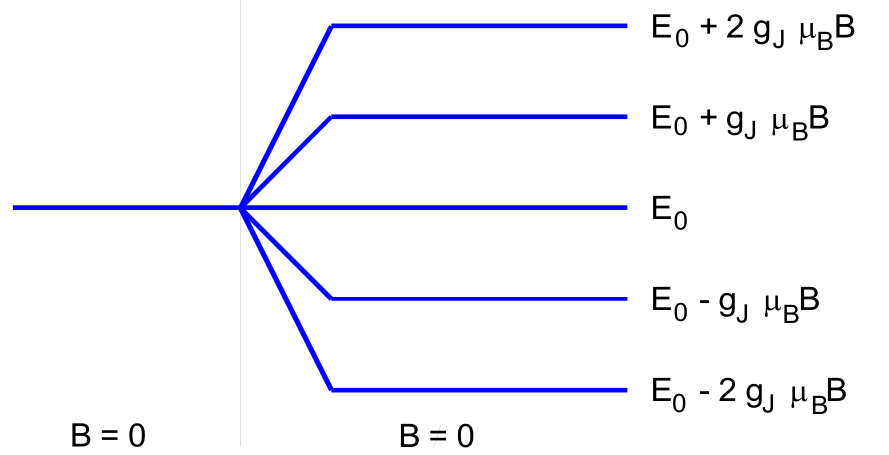
\includegraphics[width=9cm]{Pics/AufspaltungJ2.png}
  \caption{Aufspaltung der Energienievaus bei einem Atom mit J=2. \cite{anleitung01}}
  \label{fig:AufspaltungJ2}
\end{figure}

In Abbildung \ref{fig:AufspaltungJ2} ist die Aufspaltung der Energieniveaus für
$\symup{J}=2$ dargestellt.
Da diese Aufspaltung auch bei angeregten Zuständen auftritt, wird bei dem Einschalten
des Magnetfeldes auch eine Aufspaltung der emittierten Spektrallinien erwartet.
Die Anzahl der aufgespalteten Linien wird dabei durch Auswahlregeln festgelegt,
da Übergänge nicht zwischen allen Energieniveaus möglich sind.

\subsection{Auswahlregeln für Energieübergänge}

Die grundliegende Gleichung bei der Betrachtung mittels der Quantenmechanik ist
die Schrödingergleichung. Aufgrund ihrer Linearität können mehrer Lösungen superponiert
werden. Um die Auswahregeln zu bestimmen, wird von einer Lösung mit zwei
verschiedenen Wellenfunktionen ausgegangen:

\begin{equation}
  \Psi\ua{ges}(\vec{r},t) = C\ua{\alpha}\psi\ua{\alpha}(\vec{r})\exp{-\frac{i}{\hbar}E\ua{\alpha}t}
  +  C\ua{\beta}\psi\ua{\beta}(\vec{r})\exp{-\frac{i}{\hbar}E\ua{\beta}t}.
\end{equation}

Im folgenden sollen nun die Energieübergänge zwischen diesen beiden Zuständen
untersucht werden. Die Dichteverteilung dieser Wellenfunktion ist eine zeitabhängige
Größe, welche ein Schwingung des Elektrons mit einer durch die Energiedifferenz
festgelegten Frequenz $\nu\ua{\alpha,\beta}$ beschreibt.

\begin{equation}
  \nu\ua{\alpha,\beta} := \frac{E\ua{\alpha} - E\ua{\beta}}{2}
\end{equation}

Um die Intensität der emittierten Strahlung zu berechnen, muss das durch die
Schwingung hervorgerufenen Dipolmoment des Elektrons betrachten werden. Der Beitrag des
Volumenelemts dV zu der X-Komponente des Dipols beträgt dabei

\begin{equation}
  - e\ua{0}\su{x}\psi^*\psi \su{dV}
  \label{eqn:Dipol_X}
\end{equation}

wobei der Beitrag zu Y- und Z-Komponente analog ist. Um das gesamte Dipolmoment
in diese Richtung zu berechnen, muss $\eqref{eqn:Dipol_X}$ über den gesamten
Raum integriert werden. Durch verschiedene Rechenschritte lässt sich der Beitrag
in X-Richtung zu folgender Form vereinfachen:

\begin{equation}
  D\ua{x} = - e\ua{0} \, \su{const} \, 2 \, \symbffrak{Re} \left( \int \su{x} \psi\ua{\beta}^*
  \psi\ua{\alpha} \su{dV} \exp{2 \pi i \nu\ua{\alpha,\beta}t} \right).
\end{equation}

Der Term beschreibt einen mit der Frequenz $\nu\ua{\alpha,\beta}$ schwingenden
Dipol der Quanten entsprechender Energie abstrahlt.
Die Komponenten in die beiden anderen Raumrichtungen lassen sich analog berechnen.
Um die Strahlungsemission zu berechnen wird der Poynting-Vektor mit den Matrixelementen
$x\ua{\alpha,\beta}$, $y\ua{\alpha,\beta}$ und $z\ua{\alpha,\beta}$ bestimmt, wobei
$\gamma$ den Winkel zwischen Ausbreitungsrichtung der Strahlung und Dipolmoment
beschreibt.

\begin{align}
  \su{x}\ua{\alpha,\beta} &:= \int \su{x} \psi\ua{\alpha}^*\psi\ua{\beta} \su{dV} \\
  \su{y}\ua{\alpha,\beta} &:= \int \su{y} \psi\ua{\alpha}^*\psi\ua{\beta} \su{dV} \\
  \su{z}\ua{\alpha,\beta} &:= \int \su{z} \psi\ua{\alpha}^*\psi\ua{\beta} \su{dV} \\
  \lvert \vec{S}\ua{\alpha,\beta} \rvert &= \left( \lvert x\ua{\alpha,\beta} \rvert^2
  + \lvert y\ua{\alpha,\beta} \rvert^2 + \lvert z\ua{\alpha,\beta} \rvert^2 \right)
  \sin^2{\gamma}
  \label{eqn:Poynting}
\end{align}

Als Wellenfunktion für ein Atom im Magnetfeld wird der Ansatz

\begin{equation}
  \Psi = \frac{1}{\sqrt{2\pi}}\su{R(r)\Theta(\vartheta)} e^{im\varphi}
\end{equation}

gewählt. Das Magnetfeld ist in Richtung der z-Achse ausgerichtet. Werden die einzelnen
Komponenten des Dipols untersucht, ist erkenntlich, dass die z-Komponente
nur dann nicht verschwindet, wenn $m\ua{\alpha}$ = $m\ua{\beta}$ gilt. Somit ist
die erste Auswahlregel, dass für eine nicht verschwindende Komponente in z-Richtung
die beiden Orientierungsquantenzahlen der Zustände $E\ua{\alpha}$ und $E\ua{\beta}$
gleich sein müssen.

Für die x- und y-Komponente ergeben sich analog zwei Auswahregeln, bei denen die
Dipolkomponenten nicht verschwinden. Es muss entweder $m\ua{\beta}$ = $m\ua{\alpha}$
+ 1 ($\increment m = -1$) oder $m\ua{\beta}$ = $m\ua{\alpha}$ - 1 ($\increment m = +1$)
gelten. Zusammengefasst tritt die Emission von Spektrallinien beim Zeeman-Effekt
nur dann auf, wenn sich die Orientierungsquantenzahlen der beiden Zustände
entweder gar nicht oder um ein Differenz von $\pm$1 unterscheiden.

Gilt nun $\increment m = 0$, dann ist lediglich die z-Komponente des Dipols von
Null verschieden. Der Dipol schwingt also parallel zur Magnetfeldrichtung und
emittiert linear polarisiertes Licht. Zudem strahlt der Dipol aufgrund der Winkelabängigkeit
in $\eqref{eqn:Poynting}$ nicht in Feldrichtung und besitzt seine stärkste Emission
senkrecht zu dieser.

In den Fällen $\increment m = \pm 1$ folgt beides mal $\su{z}\ua{\alpha,\beta}=0$,
wobei die x- und y-Komponenten folgenden Zusammenhang besitzen:

\begin{align}
  \su{x}\ua{\alpha,\beta} &= -i\su{y}\ua{\alpha,\beta} \;\; (\increment m = -1) \\
  \su{x}\ua{\alpha,\beta} &= i\su{y}\ua{\alpha,\beta} \;\; (\increment m = +1).
\end{align}

In beiden Fällen ergibt sich somit ein Phasenverschub von $\frac{\pi}{2}$ zwischen
x- und y-Komponente. Bei der emittierten Strahlung handelt es sich also um zirkular-
polarisiertes Licht wobei die beiden Fälle eine entgegensätzliche Drehrichtung besitzen.

\subsection{Der normale Zeeman-Effekt}

In den vorangegangenen Rechnungen wurde der Elektronenspin nicht berücksichtigt,
so dass lediglich der Fall behandelt wird, bei dem für das
Atom $S=0$ und somit $g\ua{J}=0$ gilt. Dieser Spezialfall wird historisch bedingt
Zeeman-Effekt genannt. Hier ist die Verschiebung der Energieniveaus somit
unabhängig von den Quantenzahlen L und J, so dass die Verschiebung stehts den
Wert

\begin{equation}
  \increment E = m \mu\ua{B}B \;\; \su{für} \;\; -J \leq m \leq J
  \label{eqn:EdiffZeemanNormal}
\end{equation}

besitzt. In Abbildung \ref{fig:normalerZeeman} ist diese Aufspaltung für die
Fälle $J=1$ und $J=2$ beispielhaft dargestellt.

\begin{figure}
  \centering
  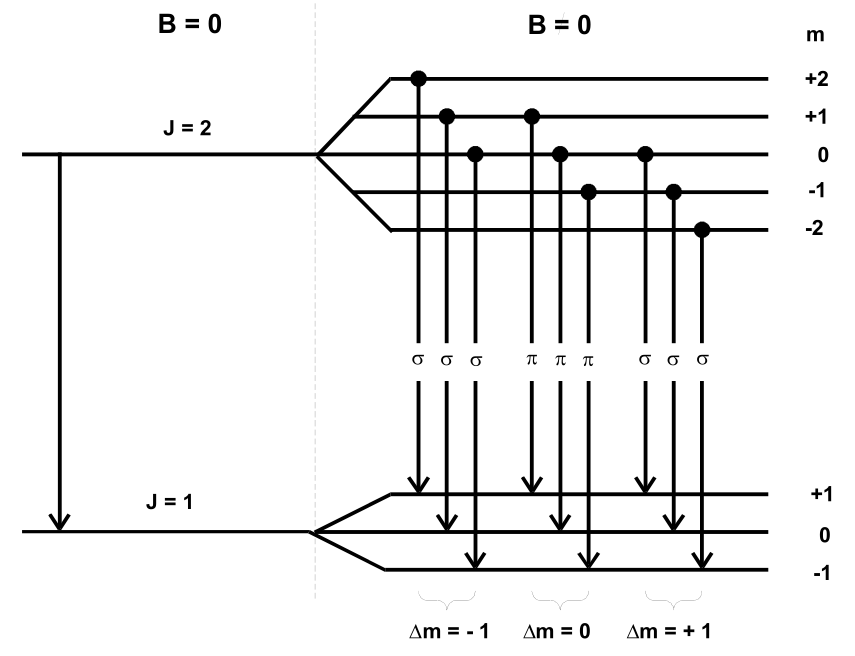
\includegraphics[width=12cm]{Pics/normalerZeeman.png}
  \caption{Aufspaltung und Polarisation der emittierten Spektrallinien beim
  normalen Zeeman-Effekt. \cite{anleitung01}}
  \label{fig:normalerZeeman}
\end{figure}

Alle Übergänge mit gleichem $\increment m$ werden in eine Liniengruppe zusammegefasst,
wobei innerhalb dieser Gruppen die Energiedifferenz konstant ist. Diese Aufspaltung
in 3 Komponenten wird auch \textbf{"Zeeman-Triplett"} genannt. Da die aufgrund des
Übergangs mit $\increment m = 0$ hervorgerufene Strahlung parallel zur Magnetfeldrichtung
linear polarisiert ist, lässt sie sich in voller Intensität nur senkrecht zur
Feldrichtung (transversal) beobachten, während sie parallel zur Feldrichtung
(longitudinal) nicht beobachtbar
ist. Gemäß Formel \eqref{eqn:EdiffZeemanNormal} ist ihre
Energie gegenüber dem feldfreien Fall nicht verändert. Sie wird als $\pi$-Komponente
bezeichnet.

Die beiden zirkular poloarisierten Linien mit $\increment m = \pm 1$ erscheinen
bei der transversalen Betrachtung linear polarisiert und können deswegen nicht
unterschieden werden. Die Linien besitzen immer ein Energiedifferenz von
$\mu\ua{B}B$ bezogen auf die unverschobenen Linien und werden als $\sigma$-Komponente
bezeichnet. Die beobachtbare Aufspaltung bei den zwei verschiedenen Betrachtungswinkeln
ist in Abbildung \ref{fig:Betrachtungswinkel} noch einmal grob dargestellt.

\begin{figure}
  \centering
  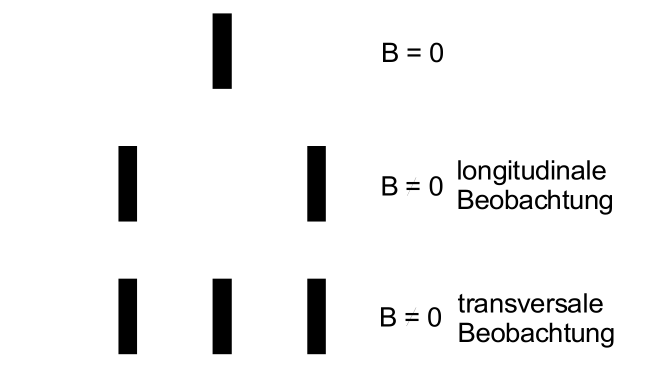
\includegraphics[width=9cm, height=5.5cm]{Pics/Betrachtung.png}
  \caption{Sichtbare Aufspaltung bei transversaler und longitudinaler Betrachtung
  der emittierten Spektrallinien. \cite{anleitung01}}
  \label{fig:Betrachtungswinkel}
\end{figure}

\subsection{Der anomale Zeeman-Effekt}

Der anomale Zeeman-Effekt beschreibt nun den in der Natur viel häufiger auftretenden
Fall von Atomen mit $S\neq0$. Die vorher hergeleiteten Auswahlregeln sind auch in
diesem Fall noch gültig, jedoch ist die Verschiebung der Energieniveaus nicht mehr
äquidistant. Für die Energie der aufgespalteten Spektrallinien ergibt sich nun
folgende Formel:

\begin{equation}
  E = \left\{ m\ua{1}g(L\ua{1},S\ua{1},J\ua{1}) - m\ua{2}g(L\ua{2},S\ua{2},J\ua{2}) \right\} \mu\ua{B}+E\ua{0}.
  \label{eqn:EdiffZeemanAnomal}
\end{equation}

Hier ist der Landé-Faktor abhängig von den Quantenzahlen $J, L $ und $S$, weswegen
die Auspaltung linienreicher wird. In Abbildung \ref{fig:AlkaliBeispiel} ist diese
Aufspaltung anhand eines Alkali-Dubletts dargestellt.

\begin{figure}
  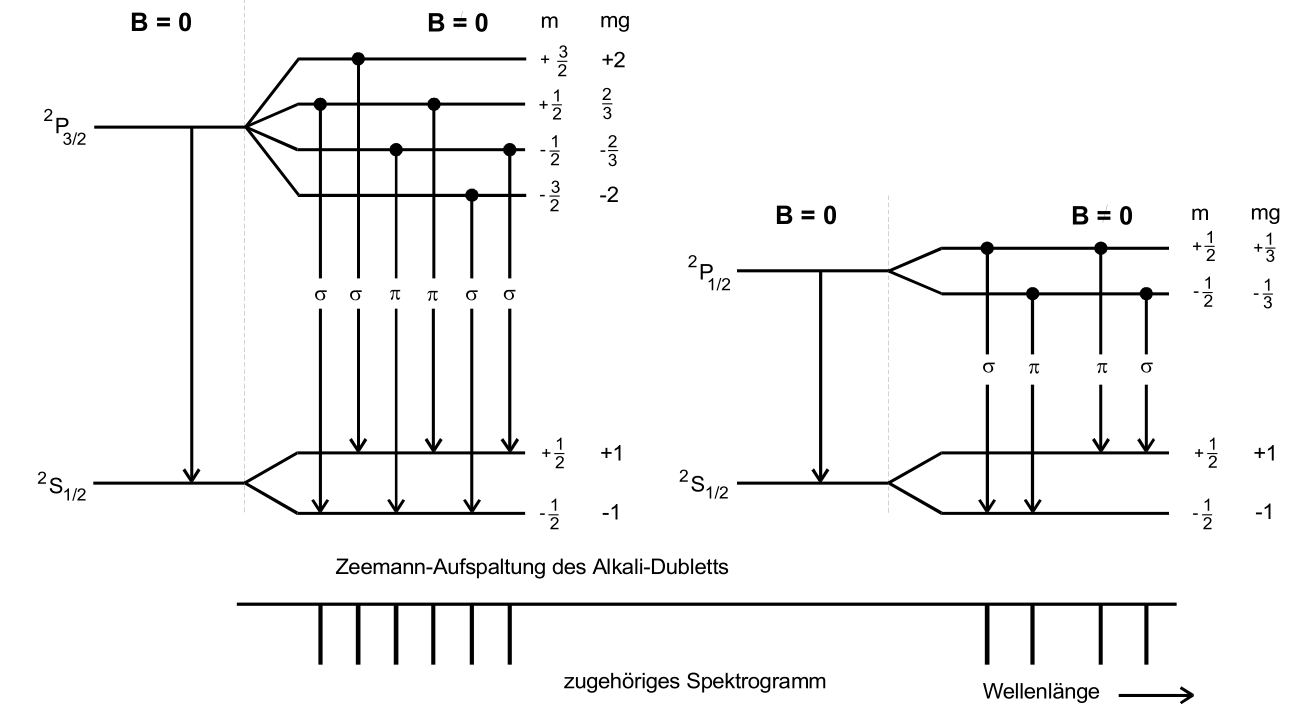
\includegraphics[width=15cm]{Pics/Alkali.png}
  \caption{Aufspaltung beim anomalen Zeeman-Effekt anhand eines Alkali-Dubletts. \cite{anleitung01}}
  \label{fig:AlkaliBeispiel}
\end{figure}

\newpage

\subsection{Die Lummer-Gehrke-Platte}

\begin{figure}
  \centering
  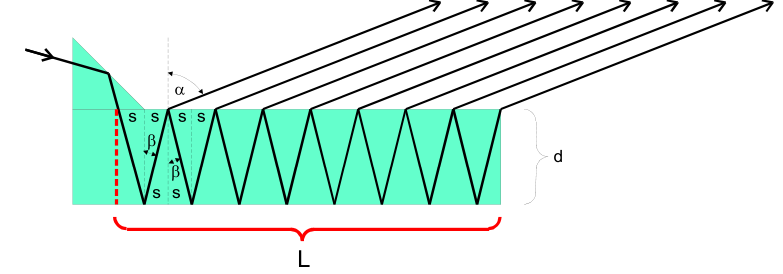
\includegraphics[width=10cm]{Pics/Lummer.png}
  \caption{Aufbau der Lummer-Gehrke-Platte. \cite{anleitung01}}
  \label{fig:LummerGehrke}
\end{figure}

Der Aufbau der Lummer-Gehrke-Platte ist in Abbildung \ref{fig:LummerGehrke} dargestellt.
Sie nutzt die Interferenz an planparallelen Platten. Das einfallende Licht wird
mittels eines Prismas in die Platte gelenkt und innerhalb dieser mehrfach
totalreflektiert. Jedoch transmittiert jedes Mal etwas Licht, da die Platte keine
perfekte Oberfläche besitzt. Die austretenden Strahlenbündel können dann miteinander
interferieren und konstruktive Interferenz erzeugen. Dafür muss jedoch die
Bedingung

\begin{equation}
  2 \cdot d \cdot \cos{\theta} = n \cdot \lambda
  \label{eqn:Bragg}
\end{equation}

mit der Plattendicke $d$ und der Wellenlänge $\lambda$ erfüllt sein. Bei
monochromatischem Licht werden Interferenzstreifen erzeugt, die genau die Wellenlänge
als Gangunterschied besitzen. Bei Einschalten des Magnetfeldes verändert sich die
Wellenlänge jedoch um $\delta\lambda$, sodass auch die Interferenzstreifen um
$\delta s$ verschoben werden. Um eine Überlagerung zweier Wellenlängen zu vermeiden,
muss die Differenz kleiner als

\begin{equation}
  \increment \lambda\ua{D} = \frac{\lambda^2}{2\cdot d} \cdot \sqrt{ \frac{1}{n^2-1}}
  \label{eqn:DispersionsLambda}
\end{equation}

sein (Dispersionsgebiet). Für die Lummer-Gehrke-Platte kann zudem abhänig vom
Brechungsindex n, der Länge L und der Wellenlänge des verwendeten Lichts ein
Auflösungsvermögen definiert werden:

\begin{equation}
  A = \frac{\lambda}{\increment\lambda} = \frac{L}{\lambda} \left( n^2-1 \right).
  \label{eqn:Auflösungsvermögen}
\end{equation}


\newpage

\section{Versuchaufbau und Durchführung}

\subsection{Aufbau}

\begin{figure}
  \centering
  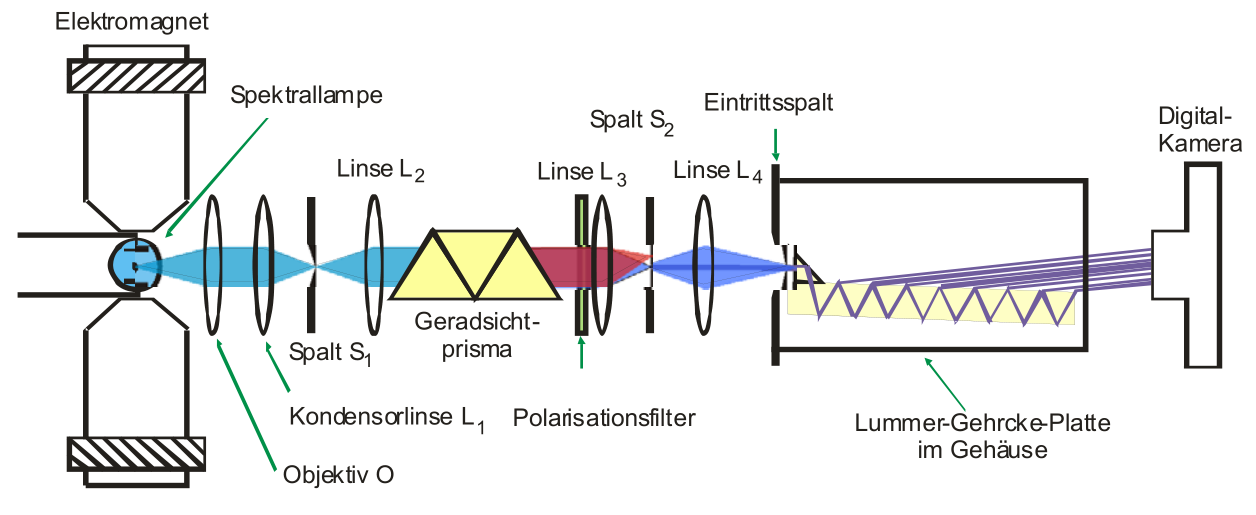
\includegraphics[width=15cm]{Pics/Aufbau.png}
  \caption{Experimenteller Aufbau zur Untersuchung des Zeeman-Effektes. \cite{anleitung01}}
  \label{fig:Aufbau}
\end{figure}

Der experimentelle Aufbau ist in Abbildung \ref{fig:Aufbau} zu sehen. Zur Betrachtung
des Zeeman-Effektes wird bei diesem Versuch eine Cadmium-Lampe verwendet. Mit der
roten Spektrallinie soll der normale und mit der blauen der anomale Zeeman-Effekt
untersucht werden. Die Cd-Lampe befindet sich zwischen den Polschuhen eines Elektromagneten,
welche von einem Generator versorgt wird. Durch ein Objektiv und ein Linsensystem
aus zwei bündelden Linsen und einem Spalt wird das in transversale Richtung emittierte
Licht kollimiert und anschließend auf ein Gradsichtprisma gebracht. Hier wird das
Licht nach der Wellenlänge separiert, sodass die zu untersuchende Spektrallinie
anschließend mittels eines Spaltes abseparieren werden kann. Nach Durchlauf des Polarisationsfilters
wird die Spektrallinie auf die Eintrittsfläche eine Lummer-Gehrke-Platte projeziert.
Diese erzeugt dann ein Interferenzmuster, welches mit einer Digitalkamera aufgenommen
wird.

\subsection{Vorbereitende Berechnungen}

Zur Vorbereitung des Versuches werden die Termschemata für die rote (\ce{^{1}P_{1}}
$\leftrightarrow$ \ce{^{1}D_{2}}) und die blaue (\ce{^{3}S_{1}} $\leftrightarrow$ \ce{^{3}P_{1}})
genauer Untersucht. Das Termschema der roten Spektrallinie zur Betrachtung des
normalen Zeeman-Effektes ist in Abbildung \ref{fig:TermschemaRot} dargestellt.
Zudem werden die Landé-Faktoren der Übergänge mithilfe
von Formel \eqref{eqn:LandéNormal} berechnet (Tabelle \ref{tab:LandéRot}).
Unter der Annahme, dass S=0
und somit J=L gilt, vereinfacht sich diese Formel zu einem konstanten Wert
von $g_J = 1$.
Der Landé-Faktor des Überganges ist durch die folgende Formel gegeben:

\begin{equation}
  g\ua{12} = m_1g_1 - m_2g_2.
  \label{eqn:Landékomplett}
\end{equation}

Bei der roten Spektrallinie vereinfacht sich dies zu $g\ua{12} = m_1 - m_2$.

\begin{figure}
  \centering
  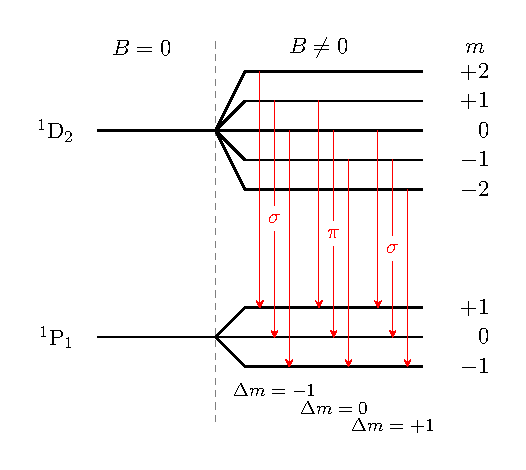
\includegraphics[width=0.7\textwidth]{Pics/termschema_rot.pdf}
  \caption{Termschema zum Übergang \ce{^{1}P_{1}} $\leftrightarrow$ \ce{^{1}D_{2}}
          \cite{luckyjosh}.}
  \label{fig:TermschemaRot}
\end{figure}

\begin{table}
	\centering
  \caption{Landé-Faktoren für den Übergang \ce{^{1}P_{1}} $\leftrightarrow$ \ce{^{1}D_{2}}.}
	\label{tab:LandéRot}
	\begin{tabular}{cccccc}
		\toprule
		{} & \multicolumn{2}{c}{${}^1P_1$}  & \multicolumn{2}{c}{${}^1D_2$}  & $^1P_1\leftrightarrow ^1\!\!D_2$ \\
		\midrule
		 Übergang &   $m_1$  & $g_{1}$ & $m_2$ & $ g_2$  & $g_{12}$  \\
		\midrule
		& 2 & 1 & 1 & 1 & 1\\
		$\sigma$& 1 & 1 & 0 & 1 & 1\\
		& 0 & 1 & -1 & 1 & 1\\
		\midrule
		& 1 & 1 & 1 & 1 & 0\\
		$\pi$ & 0 & 1 & 0 & 1 & 0\\
		& -1 & 1 & -1 & 1 & 0\\
		\midrule
		& 0 & 1 & 1 & 1 & -1\\
		$\sigma$ & -1 & 1 & 0 & 1 & -1\\
		& -2 & 1 & -1 & 1 & -1\\\bottomrule
	\end{tabular}
\end{table}

Für die blaue Spektrallinie (\ce{^3S_1} $\leftrightarrow$ \ce{^3P_1}) werden die
Landé-Faktoren ebenfalls mit Formel \eqref{eqn:LandéNormal} berechnet, jedoch wird
bei dem anomalen Zeeman-Effekt der Spin beachtet, sodass sich diese Formel nicht
weiter vereinfachen lässt (Tabelle \ref{tab:Landé_blau}). Das zugehörige Termschema
ist in Abbildung \ref{fig:termschema_blau} zu sehen. Der gemischte Landé-Faktor
ergibt sich hier nach Formel \eqref{eqn:Landékomplett}.

\begin{figure}[h]
  \centering
  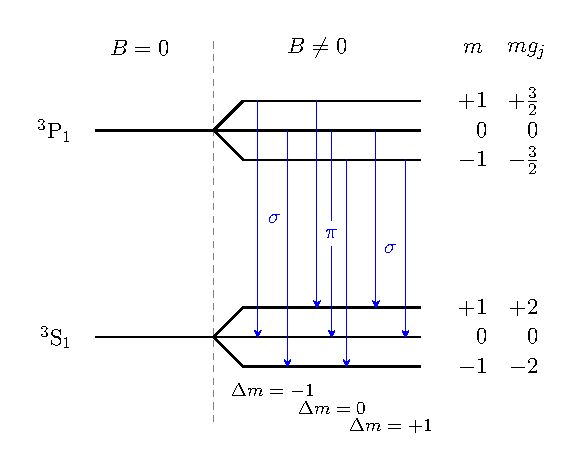
\includegraphics[width=0.7\textwidth]{Pics/termschema_blau.pdf}
  \caption{Termschema für den Übergang \ce{^3S_1} $\leftrightarrow$ \ce{^3P_1} \cite{luckyjosh}.}
  \label{fig:termschema_blau}
\end{figure}

\begin{table}

  \caption{Landé-Faktoren für den Übergang \ce{^3S_1} $\leftrightarrow$ \ce{^3P_1}. }
	\label{tab:Landé_blau}
	\centering
  \renewcommand{\arraystretch}{1.2}
  \begin{tabular}{cccccc}
		\toprule
    & \multicolumn{2}{c}{${}^3S_1$}  & \multicolumn{2}{c}{${}^3P_2$} \\
		\midrule
    Übergang & $m_1$  & $g_{1}$ & $m_2$ & $ g_2$ & $g_{12}$\\
		\midrule
		$\sigma$ & +1 & 2 & 0 & $\frac{3}{2}$& 2\\
		& 0 & 2 & -1 & $\frac{3}{2}$ & $\frac{3}{2}$\\
		\midrule
		& +1 & 2 & +1 & $\frac{3}{2}$ & $\frac{1}{2}$\\
		$\pi$ & 2 & 2 & 0 & $\frac{3}{2}$ & 0 \\
		& -1 & 2 & -1 & $\frac{3}{2}$ & -$\frac{1}{2}$\\
		\midrule
		& 0 & 2 & 1 & $\frac{3}{2}$ & -$\frac{3}{2}$\\
		$\sigma$ & -1 & 2 & 0 & $\frac{3}{2}$& -2\\
		\bottomrule
	\end{tabular}
\end{table}

Die Energiedifferenz der aufgespalteten Linien lässt sich mit
$\increment E = g\ua{12} \mu\ua{B} B$ berechnen.

Im letzten Teil der Vorbereitung wird das Auflösungsvermögen, sowie
das Dispersionsgebiet beider Übergänge mit den Formeln \eqref{eqn:DispersionsLambda}
und \eqref{eqn:Auflösungsvermögen} berechnet.

\begin{align}
  & \ce{^{1}P_{1}} \leftrightarrow \ce{^{1}D_{2}}: \quad \quad \lambda=\SI{643.8}{\nano\meter} \notag\\
  & A \approx 209128.6, \quad \Delta \lambda \approx \SI{4.98e-11}{\meter}  \\ % (\SI{643.8}{\nano\meter})
  & \ce{^3S_1} \leftrightarrow \ce{^3P_1}: \quad \quad \lambda=\SI{480.0}{\nano\meter}\notag \\
  & A \approx 285458, \quad \Delta \lambda \approx \SI{2.7e-11}{\meter}. % (\SI{480.0}{\nano\meter})
\end{align}


\subsection{Durchführung}

Zu Beginn des Experimentes wird zuerst eine Hysterekurve des verwendeten Elektromagneten
aufgenommen. Dafür wird das Magnetfeld für verschiedene Stromstärken in einem Bereich
von 0 bis 20 A gemessen, mit einer Differenz von 1 A der verschiedenen Messwerte.
Es wird eine Messreihe beim Aufdrehen und eine beim Runterregeln des Stromes aufgenommen.

Danach wird die Apperatur für die Messungen justiert. Zuerst werden das Objektiv
und die Kondensorlinse $L\ua{1}$ so verschoben, dass die Cd-Lampe scharf auf den
Spalt $S\ua{1}$ abgebildet wird. Danach wird mittels der Linse $L\ua{2}$ ein
paralleles Lichtbündel auf das Gradsichtprisma geworfen. Dabei soll
möglichst wenig Strahlung verloren gehen, indem der Durchmesser des Bündels nicht
größer als die Eintrittsfläche des Prismas eingestellt wird. Anschließend wird mit
der Linse $L\ua{3}$ das Licht erneut gebündelt und auf den anschließende Spalt $S\ua{2}$
projeziert. Dieser wird so eingestellt, dass die rote Spektrallinie rausgefiltert wird.
Nach Durchlaufen einer weitern Sammellinse $L\ua{4}$ und des Polarisationsfilters wird
die separierte Spektrallinie auf das Eintrittsprisma der Lummer-Gehrke-Platte geworfen.
Dabei wird die Platte so verschoben, dass kein Licht direkt auf die Platte fällt
oder am Eintrittsprisma vorbeigeht. Mit der Kamera kann das entstehende
Interferenzmuster mittels einiger Einstellungen bezüglich des Fokusses und der
Belichtungszeit aufgenommen werden.

Zuerst wird Das Interferenzmuster bei ausgeschaltetem Magnetfeld und einer
Belichtungszeit von 8 Sekunden aufgenommen. Anschließend wird der Polarisationsfilter
so eingestellt, dass der Fall $\increment m = \pm 1$ beobachtet werden kann. Das
Magnetfeld wird solange aufgedreht, bis eine Aufspaltung der Spektrallinien
beobachtbar ist. Anschließend wird der Polarisationsfilter um $\frac{\pi}{2}$ gedreht,
sodass die Spektrallinie für $\increment m = 0$ aufgenommen werden kann.

Um den anomalen Zeeman-Effekt beobachten zu können, wird der Spalt $S\ua{2}$ so
verschoben, dass die hellblaue Spektrallinier herausgefiltert wird. Danach wird
wie im vorherigen Verlauf die Lummer-Gehrke-Platte justiert. Zuerst wird eine
Aufnahme des Interferenzmusters bei ausgeschaltetem Magnetfeld angefertigt.
Durch Aufdrehen des Magnetfeldes und geeigneter Einstellung des Polarisationsfilters
kann dann die Aufspaltung für den Fall $\increment m = \pm 1$ beobachtet werden.
Zuletzt wird der Polarisationsfilter wieder gedreht und die Stromstärke so lange
erhöht, bis auch die Aufspaltung im Fall $\increment m = 0$ sichtbar ist. Alle
Aufnahmen werden ebenfalls mit einer Belichtungszeit von 8 Sekunden angefertigt.
